%%% -*- mode:latex; mode:flyspell -*-

%%% Local Variables:
%%% TeX-master: "mu2e-36575"
%%% End:
\section{Tuning the calorimeter timing resolution}

The calorimeter timing simulation has been significantly improved since the Offline version that was \strike{freezed} {\blue frozen}
to build the SU2020 repository.
\strike{\textbackslash n}
The old timing {\blue simulation} was largely underestimating the calorimeter tim\strike{e}{\blue ing} resolution. A better 
parametrization of the photon propagation time inside the crystal and, most significantly, a better implementation of the noise in
the simulation {\blue in more recent versions of the Offline produces} \strike{now makes the} simulation results much closer to the test 
beam measurements \cite{MU2E_35540_CALO_TIMING}.

The different components of the calorimeter noise during the first period of data taking have been estimated in \cite{MU2E_35519_CALO_NOISE}
assuming the Run Plan reported in \cite{MU2E_33731_RUN1_PLAN}\strike{. T}{\blue , where t}he results are summarized in 
\strike{t}{\blue T}able \ref{table:calonoise}.
\strike{They}{\blue The noise components} include {\blue the} electronic noise (measured at {\blue the} cosmic ray\strike{s} stand), 
\strike{the} {\blue r}\strike{R}adiation  {\blue i}\strike{I}nduce{\blue d n}\strike{N}oise (RIN){\blue ,} and \strike{the} {\blue d}\strike{D}ark
{\blue c}\strike{C}urrent
produced by \strike{the} neutron radiation damage in the SiPMs (assuming \strike{to operate them at}{\blue an operation temperature of} $-10^o$ C).
A safety factor {\blue of} 2 has been used for the  neutron induced noise to reflect the uncertainty of the results of neutron radiation damage
measurements.

\begin{table}[htbp]
  \begin{center} 
    \begin{tabular}{|c|c|c|c|c|}
      \hline
      Run 1 \strike{Time}{\blue era} & FEE noise  & RIN     &  Dark {\blue current or name dark noise above} \strike{Noise} & Total    \\ 
      \hline
      1 batch start     & 200 keV    & 280 keV &  --         & 344 keV  \\
      1 batch end       & 200 keV    & 280 keV &  450 keV    & 566 keV  \\
      2 {\blue batch}\strike{bacthes} end     & 200 keV    & 400 keV &  492 keV    & 634 keV  \\
      \hline
    \end{tabular}
  \end{center}
  \caption{
  \label{table:calonoise}
    Calorimeter noise levels in different {\blue eras} \strike{moments} of Run 1 as estimated in \cite{MU2E_35519_CALO_NOISE}.
  }
  % \vspace{0.5in}
\end{table}

Using the result{\blue s} in the \strike{table} {\blue Table \ref{table:calonoise},} we assume an average noise of 455 keV for the 1 batch period
and 600 keV for the 2 batch\strike{es} period. \strike{\textbackslash n}
A parametrization of the time resolution as function of the noise level and the energy deposited in a crystal obtained using the latest calorimeter 
simulation software has been presented in \cite{MU2E_36225_CALO_TIME_RES}. The curves corresponding to 455 keV and 600 keV {\blue noise levels} are
the lower dashed lines in {\blue F}\strike{f}igures \ref{fig:calorimeter_timing_resolution_1batch} and \ref{fig:calorimeter_timing_resolution_2batch}.

Table \ref{table:calonoise} \strike{doesn't} {\blue does not} include the time jitter of the accelerator signal. This effect should also be included 
in the tracker timing  simulation{\blue , where it is currently ignored}. For particle identification{\blue ,} the only relevant quantity is 
the relative time between {\blue the} tracker and calorimeter. 
We decided not to change the tracker timing simulation\strike{ and}{\blue, but instead} to add the accelerator clock jitter \strike{all} {\blue only}
to the cluster time.
Preliminary measurements \cite{MU2E_35392_TIME_JITTER} show a time jitter of 172 ps for 2 DTCs in chain and 217 ps for 7 DTCs in chain. 
We take 200 ps as our best \strike{guess} {\blue estimate}.

\strike{Being the update of calorimeter software a too big modification for the SU2020 software repository and aiming to include also the effect of the DTCs 
time jitter we have modified the CaloCrystalHitFromHit module adding an additional time gaussian smearing to reproduce the wanted time resolution.}
{\blue The update to the calorimeter software is too complex to be imported to the SU2020 software repository. Instead, an additional Gaussian time smearing
component is added to the CaloCrystalHitFromHist module to reproduce the desired time resolution.}
\strike{\textbackslash n}
Figures \ref{fig:calorimeter_timing_resolution_1batch} and \ref{fig:calorimeter_timing_resolution_2batch} show the output of the 
\strike{pacthed} time resolution simulation {\blue with the additional Gaussian smearing component} as {\blue a} function of the energy deposited in the
crystal for the two calorimeter disks \strike{in case of 1 or 2 proton bacthes.} {\blue for 1 and 2 batch modes.} The agreement with the expected analytical
function is shown. The deviations at small energies are not \strike{relevant because} {\blue important as} the time resolution simulation in those regions
is known to be less reliable.

\begin{figure}[h]
  \hspace{-0.6in}
  \begin{tikzpicture}
    \node[anchor=south west,inner sep=0] at (-1,0.) {
      % \node[shift={(0 cm,0.cm)},inner sep=0,rotate={90}] at (0,0) {}
      \makebox[\textwidth][c] {
        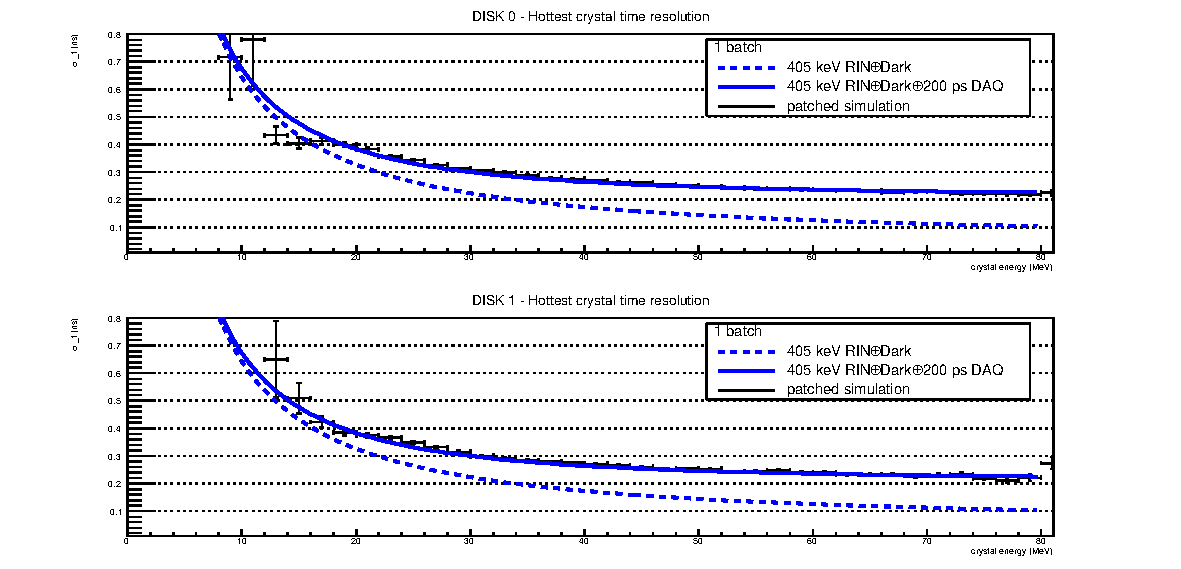
\includegraphics[width=0.80\textwidth]{figures/pdf/figure_00401_sigmat_1batch_corrected}
      }
    };
    % \node [text width=6cm, scale=0.8] at (4.5,6.4) {mu2e-18894 by Kevin Lynch and Jim Popp};
  \end{tikzpicture}
  % \captionof{figure} {
  \caption{
    \label{fig:calorimeter_timing_resolution_1batch}
    Tuning of {\blue the} calorimeter timing resolution for the 1 batch run period. The lower dashed curve corresponds to the parametrization given in 
    \cite{MU2E_36225_CALO_TIME_RES} \strike{applying} {\blue using} a noise of 455 keV. The upper dashed curve includes the 200 ps for the DTCs time 
    \strike{hitter} {\blue jitter}. The black points represent the result{\blue s} of the SU2020 patched calorimeter time simulation.
  }
\end{figure}

\begin{figure}[h]
  \hspace{-0.6in}
  \begin{tikzpicture}
    \node[anchor=south west,inner sep=0] at (-1,0.) {
      % \node[shift={(0 cm,0.cm)},inner sep=0,rotate={90}] at (0,0) {}
      \makebox[\textwidth][c] {
        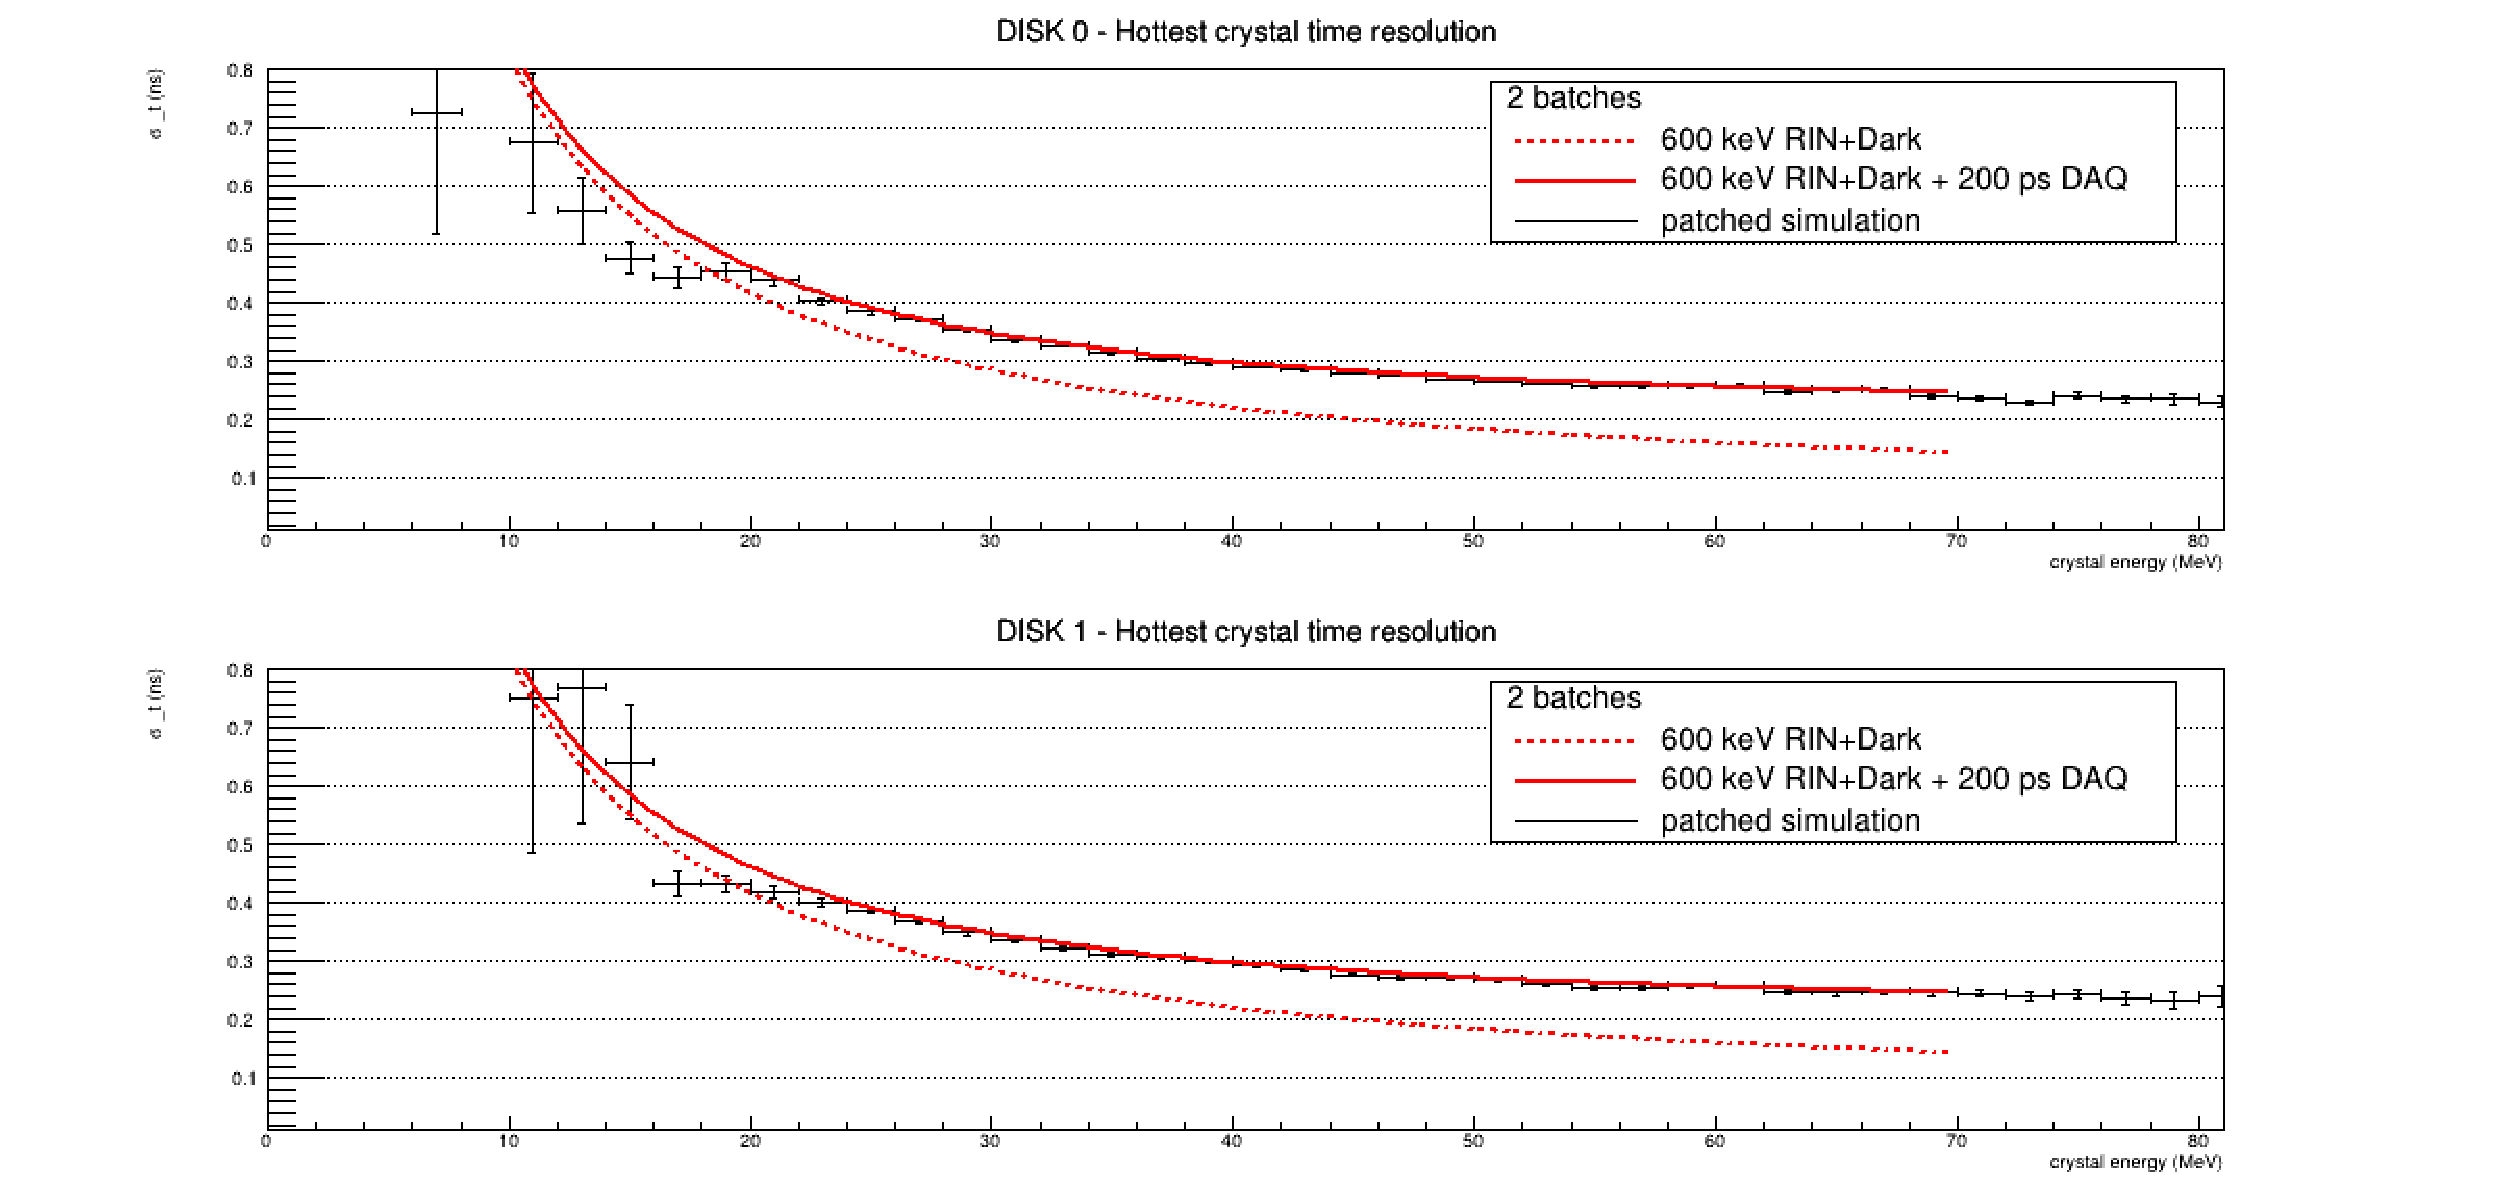
\includegraphics[width=0.80\textwidth]{figures/pdf/figure_00402_sigmat_2batch_corrected}
      }
    };
    % \node [text width=6cm, scale=0.8] at (4.5,6.4) {mu2e-18894 by Kevin Lynch and Jim Popp};
  \end{tikzpicture}
  % \captionof{figure} {
  \caption{
    \label{fig:calorimeter_timing_resolution_2batch}
    Tuning of {\blue the} calorimeter timing resolution for the 2 batch\strike{es} run period. The lower dashed curve corresponds to the parametrization
    given in \cite{MU2E_36225_CALO_TIME_RES} \strike{applying} {\blue using} a noise of 600 keV. The upper dashed curve includes the 200 ps for the DTCs
    time \strike{hitter} {\blue jitter}. The black points represent the result{\blue s} of the SU2020 patched calorimeter time simulation. 
  }
\end{figure}
